% Volume III: Probability, Statistics, Information, and Causality
% Continuity note for Chapter 14.
% Previous dependencies: Chapter 13's probability spaces, random variables as functions, induced distributions, joint/marginal/conditional distributions, random vectors, mean vectors, covariance matrices, and covariance ellipses.
% New durable concepts: probability mass function; probability density; support; parameter; data-generating story; Bernoulli, categorical, binomial, geometric, Poisson, uniform, Gaussian, exponential, gamma, beta, and multivariate Gaussian distributions; precision matrix; Mahalanobis distance; exponential-family form; sufficient statistic; natural parameter; log-partition function; mean-parameter identities; GLM link functions.
% Forward hooks: Chapter 15 reuses these distributions inside expectations, conditioning, and Bayes updates; Chapter 16 reuses binomial, Poisson, Gaussian, and sample-mean behavior in limit theorems; Chapter 17 reuses likelihoods, sufficient statistics, Fisher information, and maximum-likelihood estimation; Chapter 18 reuses exponential-family geometry, entropy, KL divergence, and Fisher geometry.
% Notation commitments: Random variables are uppercase X,Y,N,K,T; realized values are lowercase x,y,n,k,t; discrete mass functions use p_X(x)=P(X=x); continuous densities use p_X(x) with probabilities computed by integration; parameters are p, \pi, n, \lambda, \mu, \sigma^2, \alpha, \beta, and \Sigma; multivariate Gaussians use X\sim\mathcal N(\mu,\Sigma) with precision \Lambda=\Sigma^{-1}; exponential families use p(x\mid \eta)=h(x)\exp(\eta^\top T(x)-A(\eta)).
% Figure plan: four chapter-specific raster figures under imagegen-figures/ch14-* are referenced: discrete distribution catalog for 14.1; continuous density areas for 14.2; multivariate Gaussian ellipses for 14.3; exponential-family map for 14.4.
\section{Chapter 14: Distributions and Exponential Families}
\label{ch:distributions-exponential-families}

Chapter 13 made uncertainty precise by defining probability spaces, random variables, random vectors, and covariance. A random variable is a function from outcomes to values. Its \emph{distribution} is the induced pattern of probability on those values. Chapter 14 asks how to choose and understand those patterns.

A distribution should not feel like a formula pulled from a table. It is a compact story about how data could have been generated. A Bernoulli random variable records one success-or-failure trial. A Poisson random variable counts events in a window. A Gaussian random variable models noisy variation around a mean. An exponential family explains why many such models share the same algebra.

\paragraph{Chapter problem.}
How can we recognize the right distributional model for classes, counts, waiting times, real-valued measurements, and correlated vectors, while keeping track of support, parameters, sufficient statistics, and likelihood structure?

\paragraph{Section map.}
Section 14.1 introduces core discrete distributions through probability mass functions and count-based stories. Section 14.2 introduces core continuous distributions through densities, support, and probability as area. Section 14.3 develops the multivariate Gaussian as the central model for correlated random vectors. Section 14.4 unifies many of the earlier examples as exponential families, preparing the likelihoods, Bayes updates, GLMs, and information geometry used later.

\subsection{14.1 Core discrete distributions}

\paragraph{Motivating question.}
When the observation is a label, a success count, a first-success time, or a spike count, which discrete distribution encodes the data-generating story?

\paragraph{Beginner setup.}
A \emph{discrete random variable} takes values in a finite or countably infinite set. Its distribution is described by a \emph{probability mass function}, or PMF:
\[
p_X(k)=P(X=k).
\]
The smallest nontrivial example is a Bernoulli random variable:
\[
X=
\begin{cases}
1, & \text{success},\\
0, & \text{failure},
\end{cases}
\qquad
P(X=1)=p,\quad P(X=0)=1-p.
\]
The number \(p\) is a parameter: it is not the observed value, but a property of the mechanism producing observations.

Discrete distributions solve a modeling problem. They let us convert a verbal data-generating story into a normalized assignment of probabilities over possible outcomes. A class label needs probabilities over classes. A count of successes in \(n\) trials needs probabilities over \(0,1,\ldots,n\). A spike count in a fixed time bin needs probabilities over \(0,1,2,\ldots\).

What to keep in mind: the support is part of the model. A Bernoulli random variable cannot produce \(2\). A binomial random variable with \(n=10\) cannot produce \(17\). A Poisson random variable can produce any nonnegative integer, but it assumes a single rate parameter controls both the mean and the variance. Choosing a discrete distribution starts by asking what outcomes are even possible.

\begin{figure}[htbp]
\centering
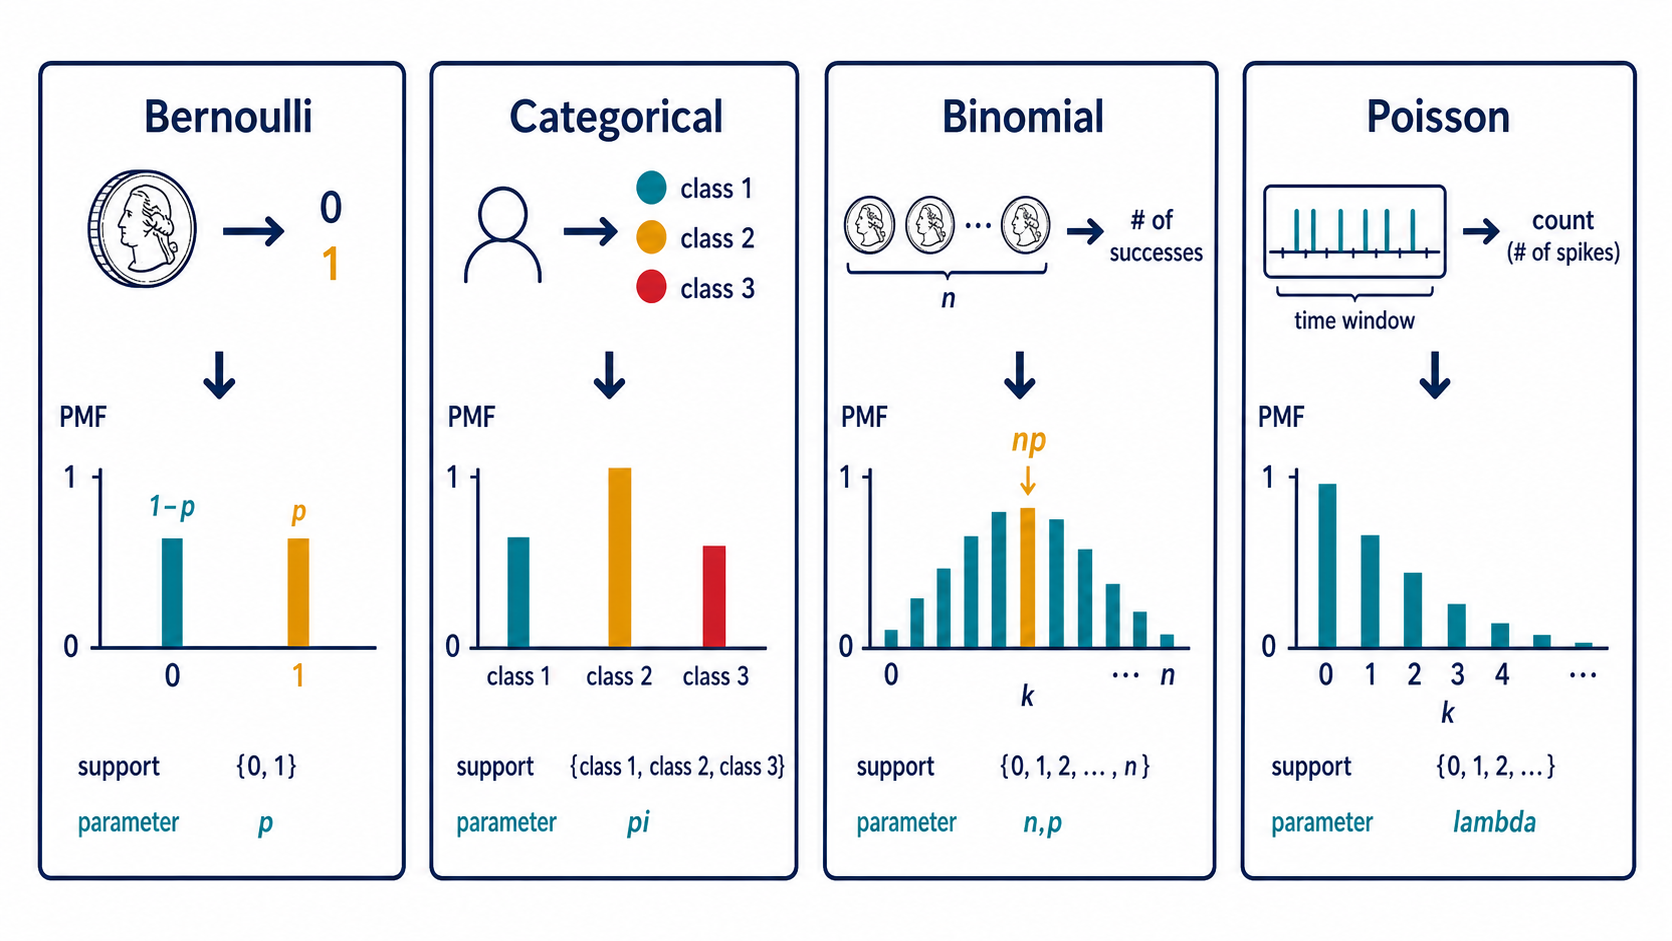
\includegraphics[width=0.98\linewidth]{imagegen-figures/ch14-discrete-distribution-catalog.png}
\caption{Core discrete distributions are best remembered by their stories and supports. Bernoulli models one binary trial; categorical models one class choice; binomial models the number of successes in \(n\) independent Bernoulli trials; Poisson models counts in a fixed window. The vertical bars are probability masses, so their total height-sum is \(1\).}
\label{fig:ch14-discrete-catalog}
\end{figure}

\paragraph{Formal setup.}
Let \(X\) be a discrete random variable with support \(\mathcal X\). A PMF is a function \(p_X:\mathcal X\to[0,1]\) satisfying
\[
\boxed{\sum_{x\in\mathcal X} p_X(x)=1,\qquad p_X(x)=P(X=x).}
\]
For a function \(g\), the expectation is
\[
E[g(X)]=\sum_{x\in\mathcal X} g(x)p_X(x),
\]
which Chapter 15 studies in detail. For now, expectations give useful summaries such as means and variances.

\begin{center}
\small
\setlength{\tabcolsep}{2pt}
\renewcommand{\arraystretch}{1.22}
\begin{tabular}{p{0.14\linewidth}p{0.16\linewidth}p{0.25\linewidth}p{0.13\linewidth}p{0.13\linewidth}p{0.12\linewidth}}
\toprule
Distribution & Story & PMF & Parameters & Mean & Variance \\
\midrule
Bernoulli & one binary trial & \(P(X=x)=p^x(1-p)^{1-x}\), \(x\in\{0,1\}\) & \(0\leq p\leq1\) & \(p\) & \(p(1-p)\) \\
Categorical & one of \(K\) classes & \(P(X=k)=\pi_k\), \(k=1,\ldots,K\) & \(\pi_k\geq0,\ \sum_k\pi_k=1\) & depends on encoding & depends on encoding \\
Binomial & successes in \(n\) independent trials & \(P(X=k)=\binom nk p^k(1-p)^{n-k}\) & \(n,\ p\) & \(np\) & \(np(1-p)\) \\
Geometric & trial number of first success & \(P(X=k)=(1-p)^{k-1}p,\ k\geq1\) & \(0<p\leq1\) & \(1/p\) & \((1-p)/p^2\) \\
Poisson & event count in a fixed window & \(P(X=k)=e^{-\lambda}\lambda^k/k!\), \(k\geq0\) & \(\lambda>0\) & \(\lambda\) & \(\lambda\) \\
\bottomrule
\end{tabular}
\end{center}

The categorical distribution is often represented with a one-hot vector \(Y\in\{e_1,\ldots,e_K\}\), where \(P(Y=e_k)=\pi_k\). In that encoding, \(E[Y]=\pi\), so the probability vector is also the mean one-hot vector.

\paragraph{Core intuition.}
Figure~\ref{fig:ch14-discrete-catalog} separates the distributions by what is being observed. A Bernoulli observation is one bit. A categorical observation is one choice among named classes. A binomial observation is an aggregate count after a fixed number of independent trials. A geometric observation is a waiting time measured in trials. A Poisson observation is a count in a window when events are rare, roughly independent, and governed by a rate.

The bars in a PMF are not histogram estimates by themselves. The PMF is the model's probability assignment. A histogram from data may suggest a PMF, but the PMF is the idealized object. This distinction matters in neuroscience: observed spike-count histograms are noisy finite-data summaries, while a Poisson model states a probability for every possible count.

Common beginner mistakes usually involve the support or the story. First, do not use a binomial distribution unless the number of opportunities \(n\) is fixed in advance. Second, do not use a Poisson distribution merely because the outcome is a count; if there is a hard maximum, a binomial or categorical model may be more appropriate. Third, do not treat the parameter as the observation. In a Poisson model \(X\sim\mathrm{Pois}(\lambda)\), \(X\) is the random count and \(\lambda\) is the expected count.

This section reuses Chapter 13's distinction between random variables and their distributions. It prepares Chapter 15's expectation calculations, Chapter 17's likelihoods, and Section 14.4's exponential-family unification.

\paragraph{Main derivation: Poisson as a rare-event limit.}
Suppose a time window is split into \(n\) tiny subwindows. In each subwindow, an event occurs with probability \(p_n=\lambda/n\), independently of the others. Let \(X_n\) be the total number of events. Then
\[
X_n\sim\mathrm{Binomial}\left(n,\frac{\lambda}{n}\right),
\]
so
\[
P(X_n=k)
=\binom nk\left(\frac{\lambda}{n}\right)^k
\left(1-\frac{\lambda}{n}\right)^{n-k}.
\]
For fixed \(k\), rewrite the terms as
\[
P(X_n=k)
=
\frac{n(n-1)\cdots(n-k+1)}{k!}
\frac{\lambda^k}{n^k}
\left(1-\frac{\lambda}{n}\right)^n
\left(1-\frac{\lambda}{n}\right)^{-k}.
\]
As \(n\to\infty\),
\[
\frac{n(n-1)\cdots(n-k+1)}{n^k}\to1,\qquad
\left(1-\frac{\lambda}{n}\right)^n\to e^{-\lambda},
\qquad
\left(1-\frac{\lambda}{n}\right)^{-k}\to1.
\]
Therefore
\[
\boxed{P(X=k)=e^{-\lambda}\frac{\lambda^k}{k!}.}
\]
The mechanism is instructive: many tiny independent opportunities, each with a small probability, produce a count distribution controlled by the expected total number \(\lambda\). This is why the Poisson distribution is a natural first model for spike counts in short windows, photon counts, queue arrivals, and rare errors.

\paragraph{Worked examples.}
\emph{Small numerical example.} A neuron is modeled as producing \(X\sim\mathrm{Pois}(2)\) spikes in a \(100\) ms window. The probability of observing exactly \(3\) spikes is
\[
P(X=3)=e^{-2}\frac{2^3}{3!}
=e^{-2}\frac{8}{6}
\approx0.180.
\]
The mean and variance are both \(2\). If the empirical variance across many trials is much larger than \(2\), the Poisson model may be too narrow.

\emph{ML example.} A classifier assigns probabilities \(\pi=(0.70,0.20,0.10)\) to classes \(\{\text{cat},\text{dog},\text{car}\}\). If the true label is dog, the categorical likelihood is \(P(X=\text{dog})=0.20\). In one-hot notation, the observed vector is \(y=(0,1,0)\), and the model probability of the observed class is \(\pi_2\).

\emph{Neuroscience example.} For a population of neurons, a simple model might assign each neuron's spike count in a short bin as \(X_i\sim\mathrm{Pois}(\lambda_i)\), where \(\lambda_i\) depends on stimulus direction. The random variable is the observed count, the parameter \(\lambda_i\) is the predicted mean count for neuron \(i\), and the likelihood of a population response is built from the count probabilities.

\paragraph{ML/DL/neuroscience connections.}
Bernoulli distributions model binary labels, dropout masks, and yes/no behavioral responses. Categorical distributions model class labels, next-token choices, and discrete latent states. Binomial distributions model aggregate success counts, such as correct trials out of \(n\). Geometric distributions model first-success waiting times in repeated attempts. Poisson distributions model counts, including spikes in fixed time windows, event arrivals, and word counts in simple text models. In each case, the mathematical object maps directly: support describes possible observations, parameters describe the data-generating mechanism, and the PMF becomes the likelihood term used for inference or learning.

\paragraph{Exercises.}
\begin{enumerate}[label=\textbf{14.1.\arabic*.}, leftmargin=*]
\item \textbf{Mechanical.} Let \(X\sim\mathrm{Bernoulli}(0.3)\). Write \(P(X=0)\), \(P(X=1)\), \(E[X]\), and \(\operatorname{Var}(X)\).
\item \textbf{Proof or derivation.} Starting from the binomial PMF, show that \(\sum_{k=0}^n \binom nk p^k(1-p)^{n-k}=1\). State which algebraic identity you used.
\item \textbf{Numerical/computational.} Compute \(P(X=2)\) for \(X\sim\mathrm{Binomial}(5,0.4)\). Then compute \(P(Y=2)\) for \(Y\sim\mathrm{Pois}(2)\). Compare the two values.
\item \textbf{Interpretation.} A spike-count dataset has sample mean \(5\) and sample variance \(25\). What does this suggest about a simple Poisson model, and which assumption may be failing?
\item \textbf{Debug the misconception.} A student says, "A count variable should always be modeled as Poisson." Give one example of a count where binomial is more appropriate and explain why the support matters.
\end{enumerate}

\subsection{14.2 Core continuous distributions}

\paragraph{Motivating question.}
When an observation can vary continuously, how can a density assign probabilities if the probability of any exact point is zero?

\paragraph{Beginner setup.}
A \emph{continuous random variable} takes values on an interval or region of the real line. It is described by a \emph{probability density} \(p_X(x)\). Densities are not probabilities at points. Instead, probabilities are areas:
\[
P(a\leq X\leq b)=\int_a^b p_X(x)\,dx.
\]
The smallest nontrivial example is a uniform random variable on \([0,1]\):
\[
p_X(x)=
\begin{cases}
1, & 0\leq x\leq1,\\
0, & \text{otherwise}.
\end{cases}
\]
Then \(P(0.2\leq X\leq0.5)=0.3\), the area of a rectangle of width \(0.3\) and height \(1\).

Continuous distributions solve the problem of modeling measurements with more resolution than a finite set of labels or counts: voltage, reaction time, synaptic weight, loss value, latent activation, stimulus intensity, or regression residual. They also provide the noise models used in likelihoods.

What to keep in mind: a density can be larger than \(1\). Only its total area must equal \(1\). Also, for a genuinely continuous random variable, \(P(X=x)=0\) for each exact value \(x\). This does not mean exact values are impossible in a physical sense; it means probability is assigned to intervals, and measurement devices discretize reality before recording numbers.

\begin{figure}[htbp]
\centering
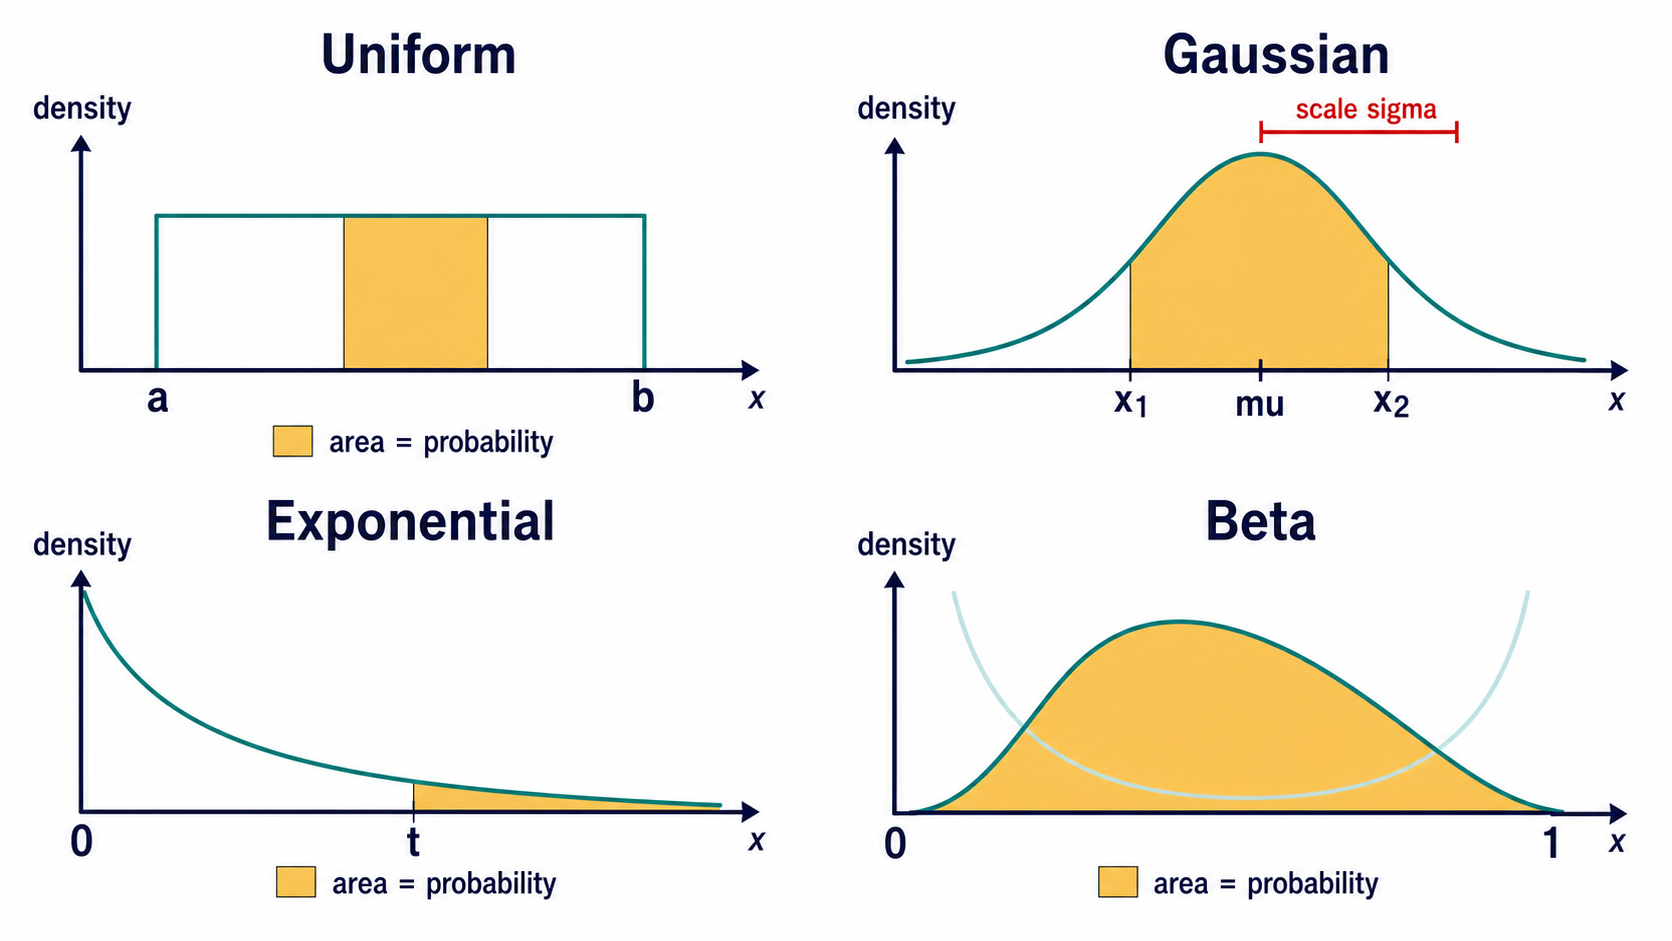
\includegraphics[width=0.98\linewidth]{imagegen-figures/ch14-continuous-density-areas.png}
\caption{Continuous distributions assign probability by area under a density curve. Uniform densities are flat on their support, Gaussian densities concentrate around a mean, exponential densities model nonnegative waiting times, and beta densities model variables constrained to \([0,1]\).}
\label{fig:ch14-continuous-density-areas}
\end{figure}

\paragraph{Formal setup.}
Let \(X\) be a continuous random variable with support \(S\subseteq\mathbb R\). A density is a nonnegative function \(p_X:S\to[0,\infty)\) satisfying
\[
\boxed{\int_S p_X(x)\,dx=1,\qquad P(X\in B)=\int_B p_X(x)\,dx.}
\]
Here \(B\subseteq S\) is an interval or measurable set. The most common continuous families in this course are:

\begin{center}
\small
\setlength{\tabcolsep}{2pt}
\renewcommand{\arraystretch}{1.22}
\begin{tabular}{p{0.14\linewidth}p{0.15\linewidth}p{0.30\linewidth}p{0.14\linewidth}p{0.15\linewidth}}
\toprule
Distribution & Support & Density & Parameters & Typical use \\
\midrule
Uniform & \([a,b]\) & \(1/(b-a)\) & \(a<b\) & bounded ignorance, random initialization intervals \\
Gaussian & \(\mathbb R\) & \(\frac{1}{\sqrt{2\pi\sigma^2}}\exp\!\left[-\frac{(x-\mu)^2}{2\sigma^2}\right]\) & \(\mu,\sigma^2>0\) & additive noise, residuals, local approximations \\
Exponential & \([0,\infty)\) & \(\lambda e^{-\lambda x}\) & \(\lambda>0\) & waiting times with constant hazard \\
Gamma & \([0,\infty)\) & \(\frac{\beta^\alpha}{\Gamma(\alpha)}x^{\alpha-1}e^{-\beta x}\) & \(\alpha,\beta>0\) & positive rates, sums of waiting times \\
Beta & \([0,1]\) & \(\frac{x^{\alpha-1}(1-x)^{\beta-1}}{B(\alpha,\beta)}\) & \(\alpha,\beta>0\) & probabilities, proportions, accuracies \\
\bottomrule
\end{tabular}
\end{center}

The Gaussian mean is \(E[X]=\mu\), and its variance is \(\sigma^2\). The exponential mean is \(1/\lambda\), and its variance is \(1/\lambda^2\). For the beta distribution,
\[
E[X]=\frac{\alpha}{\alpha+\beta},
\]
so \(\alpha\) and \(\beta\) can be read as shape parameters that pull mass toward \(1\) or \(0\).

\paragraph{Core intuition.}
Figure~\ref{fig:ch14-continuous-density-areas} shows the central geometric fact: probability is area, not height. The height \(p_X(x)\) describes how concentrated probability is near \(x\). A narrow Gaussian can have a high peak because its mass is compressed. A broad Gaussian has a lower peak because its mass is spread out.

In the Gaussian panel, the shaded probability interval runs from \(x_1\) to \(x_2\), while the separate \(\sigma\) bracket marks scale around the mean \(\mu\). These are different ideas: an interval can be chosen by the analyst, but \(\sigma\) is a parameter of the distribution.

Different continuous distributions encode different constraints. A Gaussian is convenient for real-valued deviations around a mean, but it assigns some probability to every real number. That is inappropriate for quantities that must be nonnegative, such as waiting times or firing rates. Exponential and gamma distributions live on \([0,\infty)\). A beta distribution lives on \([0,1]\), so it naturally models probabilities, proportions, or normalized behavioral accuracies.

Common misconceptions follow from confusing density with mass. First, \(p_X(2)=0.4\) does not mean \(P(X=2)=0.4\). It means the density height at \(2\) is \(0.4\). Second, the largest density value is not automatically the most probable interval unless interval widths are held fixed. Third, changing variables changes density height because probability mass must be preserved under stretching or compression, as Chapter 11's Jacobian rule explained.

This section relies on Chapter 11's integration and change-of-variables discipline. It prepares Chapter 15's expectations and Bayes updates, Chapter 16's Gaussian limit theorems, and Chapter 17's continuous likelihoods.

\paragraph{Main theorem: densities produce probabilities through cumulative area.}
Let \(X\) have density \(p_X\) on \(\mathbb R\), and define the cumulative distribution function
\[
F_X(t)=P(X\leq t)=\int_{-\infty}^t p_X(x)\,dx.
\]
Then for \(a<b\),
\[
\boxed{P(a<X\leq b)=F_X(b)-F_X(a)=\int_a^b p_X(x)\,dx.}
\]
If \(p_X\) is continuous at \(t\), then \(F_X'(t)=p_X(t)\).

\emph{Proof sketch.}
The event \(\{X\leq b\}\) can be split into two disjoint pieces:
\[
\{X\leq b\}=\{X\leq a\}\cup\{a<X\leq b\}.
\]
Additivity of probability gives
\[
F_X(b)=F_X(a)+P(a<X\leq b).
\]
Rearranging gives the interval probability. The integral form follows from the definition of the density. Finally, the fundamental theorem of calculus says that differentiating accumulated area recovers the local density when the density is continuous. The mechanism is accumulation first, local height second.

\paragraph{Worked examples.}
\emph{Small numerical example.} Let \(X\sim\mathrm{Exponential}(2)\), so \(p_X(x)=2e^{-2x}\) for \(x\geq0\). The probability that \(X\) exceeds \(1\) is
\[
P(X>1)=\int_1^\infty 2e^{-2x}\,dx=e^{-2}\approx0.135.
\]
The mean waiting time is \(1/\lambda=1/2\).

\emph{Gaussian likelihood example.} Suppose a regression model predicts a neural response amplitude \(\mu=10\), and measurement noise is modeled as Gaussian with \(\sigma=2\). For an observed response \(x=12\),
\[
p(x\mid\mu,\sigma^2)
=\frac{1}{\sqrt{2\pi(4)}}\exp\!\left[-\frac{(12-10)^2}{2(4)}\right]
=\frac{1}{2\sqrt{2\pi}}e^{-1/2}.
\]
This is a density value. A probability would require an interval, such as \(P(11.5\leq X\leq12.5)\).

\emph{Neuroscience example.} Reaction times are nonnegative and often right-skewed. A Gaussian model can assign impossible negative times and miss the skew. An exponential or gamma model respects nonnegativity, with the random variable \(T\) representing waiting time and parameters controlling the rate and shape of the distribution.

\paragraph{ML/DL/neuroscience connections.}
Gaussian densities appear as observation-noise models, variational posterior approximations, weight initializations, and local quadratic approximations to log-likelihoods. Exponential and gamma densities model nonnegative waiting times, rates, and scale parameters. Beta densities model probabilities and bounded proportions, such as accuracy, choice probability, or normalized synaptic efficacy. In all cases, the density becomes the likelihood \(p(x\mid\theta)\) of an observed continuous value under parameters \(\theta\). The support tells the model what values are legal, and the normalization integral keeps probability conserved.

\paragraph{Exercises.}
\begin{enumerate}[label=\textbf{14.2.\arabic*.}, leftmargin=*]
\item \textbf{Mechanical.} Let \(X\sim\mathrm{Uniform}(2,5)\). Write its density and compute \(P(3\leq X\leq4)\).
\item \textbf{Proof or derivation.} Verify that \(p(x)=\lambda e^{-\lambda x}\) on \([0,\infty)\) integrates to \(1\). Then derive \(P(X>t)=e^{-\lambda t}\).
\item \textbf{Numerical/computational.} For \(X\sim\mathcal N(0,1)\), use the standard normal fact \(P(-1\leq X\leq1)\approx0.6827\). What is \(P(|X|>1)\)?
\item \textbf{Interpretation.} A model uses a beta distribution for a variable \(q\). What does that tell you about the possible values of \(q\), and why might this be better than a Gaussian model for a probability?
\item \textbf{Debug the misconception.} A student says, "The density at \(x=0\) is \(1.5\), so the probability of \(X=0\) is greater than \(1\)." Explain the error.
\end{enumerate}

\subsection{14.3 Multivariate Gaussian distribution}

\paragraph{Motivating question.}
How can one distribution model several real-valued measurements at once, including their variances, correlations, and preferred directions of variation?

\paragraph{Beginner setup.}
A \emph{multivariate Gaussian} models a random vector
\[
X=(X_1,\ldots,X_d)^\top\in\mathbb R^d.
\]
It has a mean vector \(\mu\in\mathbb R^d\) and a covariance matrix \(\Sigma\in\mathbb R^{d\times d}\). The smallest nontrivial example is a two-dimensional Gaussian for two neurons' trial-to-trial firing-rate residuals after preprocessing:
\[
X=
\begin{bmatrix}
\text{neuron 1 z-scored rate residual}\\
\text{neuron 2 z-scored rate residual}
\end{bmatrix}.
\]
Raw spike counts are nonnegative integers, so they are not naturally Gaussian observations. A Gaussian model for count-derived neural data should be read as an approximation after smoothing, rate conversion, calcium-amplitude measurement, or residual/z-score preprocessing.
The diagonal entries of \(\Sigma\) are variances. The off-diagonal entries are covariances. Positive covariance means the two components tend to be high or low together.

The multivariate Gaussian solves the problem of modeling noisy real-valued vectors with a compact geometry. Instead of specifying a separate distribution for every direction, the covariance matrix tells us how variation is stretched, compressed, and tilted in space.

What to keep in mind: the covariance matrix is not just a table of pairwise facts. It defines ellipsoids of equal probability density. Its eigenvectors give the principal axes of those ellipsoids, and its eigenvalues give squared widths along those axes. This is the same spectral geometry that appeared in PCA.

\begin{figure}[htbp]
\centering
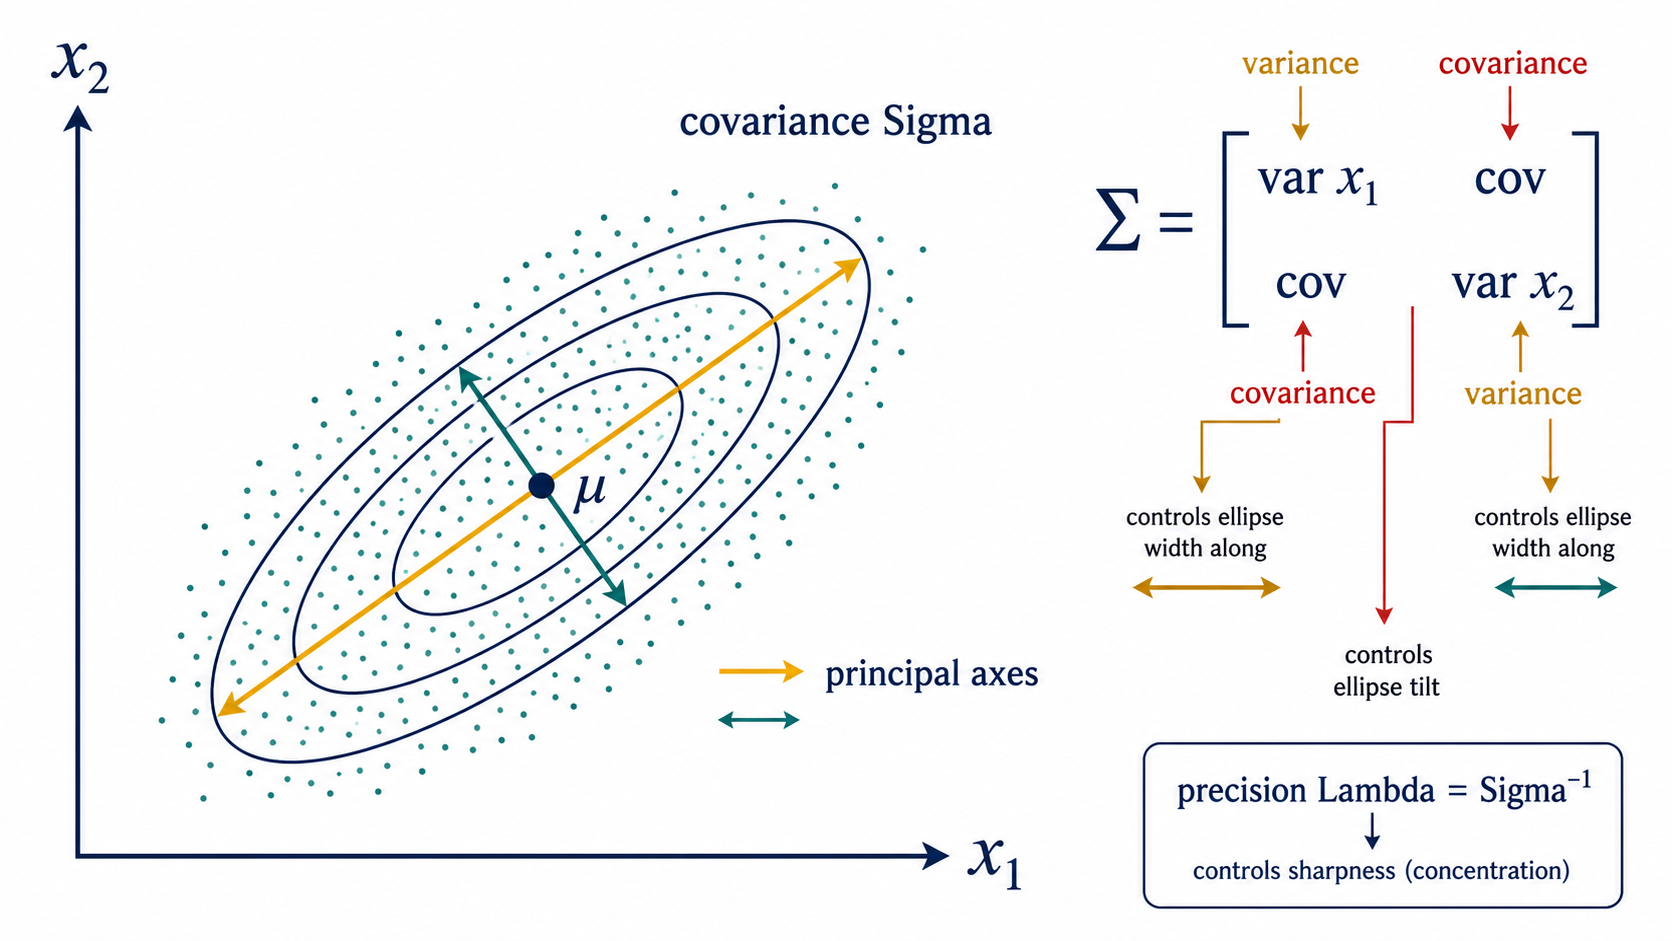
\includegraphics[width=0.98\linewidth]{imagegen-figures/ch14-multivariate-gaussian-ellipses.png}
\caption{A two-dimensional Gaussian is shaped by its mean vector and covariance matrix. The mean \(\mu\) sets the center, \(\Sigma\) sets ellipse width and tilt, and the precision matrix \(\Lambda=\Sigma^{-1}\) controls sharpness in the exponent. Positive covariance tilts the ellipses along a shared-variation direction.}
\label{fig:ch14-multivariate-gaussian}
\end{figure}

\paragraph{Formal setup.}
A random vector \(X\in\mathbb R^d\) has multivariate Gaussian distribution
\[
X\sim\mathcal N(\mu,\Sigma)
\]
when \(\mu\in\mathbb R^d\), \(\Sigma\in\mathbb R^{d\times d}\) is symmetric positive definite, and the density is
\[
\boxed{
p(x\mid\mu,\Sigma)
=
\frac{1}{(2\pi)^{d/2}|\Sigma|^{1/2}}
\exp\!\left[-\frac12(x-\mu)^\top\Sigma^{-1}(x-\mu)\right].
}
\]
The matrix
\[
\Lambda=\Sigma^{-1}
\]
is the \emph{precision matrix}. The quadratic term
\[
(x-\mu)^\top\Sigma^{-1}(x-\mu)
\]
is the squared \emph{Mahalanobis distance} from \(x\) to \(\mu\). The equal-density sets are ellipsoids:
\[
(x-\mu)^\top\Sigma^{-1}(x-\mu)=c.
\]
When \(\Sigma=I\), these sets are spheres. When \(\Sigma\) has unequal eigenvalues, they stretch into ellipsoids aligned with the eigenvectors.

\paragraph{Core intuition.}
Figure~\ref{fig:ch14-multivariate-gaussian} shows the two-dimensional case. The center is \(\mu\). The long axis marks the direction of large variance; the short axis marks the direction of small variance. If the ellipses tilt upward, then \(X_1\) and \(X_2\) are positively correlated. If the ellipses align with the coordinate axes, the covariance matrix is diagonal.

The determinant \(|\Sigma|\) measures volume scaling. A large determinant spreads mass over a larger region, so the peak density must be lower to keep total probability \(1\). The precision matrix \(\Lambda\) appears in the exponent and controls how quickly density falls away from the mean. Large precision in a direction means small variance in that direction.

Common misconceptions are important here. First, covariance and correlation are not the same: correlation is normalized covariance. Second, zero covariance does not always imply independence, but for a multivariate Gaussian it does. Third, the multivariate Gaussian is not merely "several independent Gaussians." Independence corresponds to diagonal \(\Sigma\). A full covariance matrix models coupled variation.

This section reuses Chapter 3's geometry, Chapter 6's eigenvectors and quadratic forms, Chapter 11's density normalization, and Chapter 13's covariance matrix. It prepares Gaussian conditioning in Chapter 15, concentration in Chapter 16, Fisher information in Chapter 17, and information geometry in Chapter 18.

\paragraph{Main theorem: affine transformations and Gaussian conditioning.}
Let \(Z\sim\mathcal N(0,I_d)\). If \(L\in\mathbb R^{d\times d}\) satisfies \(LL^\top=\Sigma\), then
\[
X=\mu+LZ
\]
has distribution \(\mathcal N(\mu,\Sigma)\). More generally, if \(X\sim\mathcal N(\mu,\Sigma)\), \(A\in\mathbb R^{m\times d}\), and \(b\in\mathbb R^m\), then
\[
AX+b\sim\mathcal N(A\mu+b,\ A\Sigma A^\top).
\]
If \(A\Sigma A^\top\) is singular, this should be read as a degenerate Gaussian supported on an affine subspace rather than as a full-density Gaussian on all of \(\mathbb R^m\).

If \(X\) is partitioned as
\[
X=
\begin{bmatrix}X_1\\X_2\end{bmatrix},
\qquad
\mu=
\begin{bmatrix}\mu_1\\\mu_2\end{bmatrix},
\qquad
\Sigma=
\begin{bmatrix}
\Sigma_{11} & \Sigma_{12}\\
\Sigma_{21} & \Sigma_{22}
\end{bmatrix},
\]
then the marginal distribution of \(X_1\) is
\[
X_1\sim\mathcal N(\mu_1,\Sigma_{11}),
\]
and the conditional distribution of \(X_1\) given \(X_2=x_2\) is Gaussian with
\[
E[X_1\mid X_2=x_2]
=\mu_1+\Sigma_{12}\Sigma_{22}^{-1}(x_2-\mu_2),
\]
\[
\operatorname{Cov}(X_1\mid X_2=x_2)
=\Sigma_{11}-\Sigma_{12}\Sigma_{22}^{-1}\Sigma_{21}.
\]

\emph{Proof sketch.}
For the affine transformation, use means and covariances:
\[
E[\mu+LZ]=\mu+LE[Z]=\mu,
\]
and
\[
\operatorname{Cov}(\mu+LZ)=L\operatorname{Cov}(Z)L^\top=LL^\top=\Sigma.
\]
The Gaussian family is defined so that affine transformations preserve Gaussian shape, so these moments identify the transformed Gaussian. For \(AX+b\), the same calculation gives \(A\mu+b\) and \(A\Sigma A^\top\).

For conditioning, write the joint Gaussian exponent as a quadratic form in \((x_1,x_2)\). If \(x_2\) is fixed, the terms involving \(x_1\) can be completed into a square. The center of that square is the conditional mean above, and the remaining quadratic coefficient gives the conditional covariance. The mechanism is projection: observing \(X_2\) shifts the predicted mean of \(X_1\) by the covariance-weighted residual \(x_2-\mu_2\), and it reduces uncertainty by subtracting the explained covariance.

\paragraph{Worked examples.}
\emph{Small numerical example.} Let
\[
\mu=
\begin{bmatrix}0\\0\end{bmatrix},
\qquad
\Sigma=
\begin{bmatrix}
4 & 1\\
1 & 1
\end{bmatrix}.
\]
Then \(|\Sigma|=4\cdot1-1\cdot1=3\), and
\[
\Sigma^{-1}
=\frac{1}{3}
\begin{bmatrix}
1 & -1\\
-1 & 4
\end{bmatrix}.
\]
For \(x=(2,0)^\top\), the squared Mahalanobis distance is
\[
x^\top\Sigma^{-1}x
=
\begin{bmatrix}2 & 0\end{bmatrix}
\frac{1}{3}
\begin{bmatrix}
1 & -1\\
-1 & 4
\end{bmatrix}
\begin{bmatrix}2\\0\end{bmatrix}
=\frac{4}{3}.
\]
The point \((2,0)\) is therefore closer in Mahalanobis distance than Euclidean distance alone would suggest, because the first coordinate has variance \(4\).

\emph{ML example.} In a two-dimensional latent-variable model, a latent vector \(Z\sim\mathcal N(0,I)\) may be transformed into \(X=\mu+LZ\). The matrix \(L\) maps independent latent noise into correlated observed variability. Learning \(L\) is learning the covariance geometry of the data.

\emph{Neuroscience example.} Suppose \(X_1\) and \(X_2\) are firing-rate deviations of two neurons across repeated trials. A positive off-diagonal covariance means trials with above-average activity in neuron 1 tend to have above-average activity in neuron 2. The covariance ellipse describes shared population variability, and its long axis can be compared with task-relevant coding directions.

\paragraph{ML/DL/neuroscience connections.}
The multivariate Gaussian is the default local model for random vectors because it is closed under linear transformations, marginalization, and conditioning. In ML, it appears in Gaussian discriminant analysis, Kalman filters, linear-Gaussian latent variable models, variational autoencoders with Gaussian latents, and Laplace approximations. In neuroscience, \(\mu\) can represent the mean population response to a stimulus, \(\Sigma\) the trial-to-trial population covariance, and \(\Sigma^{-1}\) the precision structure used when combining noisy cues. PCA uses the eigenvectors of empirical covariance; the multivariate Gaussian turns that covariance geometry into a full probability density.

\paragraph{Exercises.}
\begin{enumerate}[label=\textbf{14.3.\arabic*.}, leftmargin=*]
\item \textbf{Mechanical.} For \(\Sigma=\begin{bmatrix}9&0\\0&1\end{bmatrix}\), describe the orientation and relative widths of the Gaussian covariance ellipse.
\item \textbf{Proof or derivation.} If \(X\sim\mathcal N(\mu,\Sigma)\) and \(Y=AX+b\), derive \(E[Y]\) and \(\operatorname{Cov}(Y)\) from the definitions of mean and covariance.
\item \textbf{Numerical/computational.} Let \(\Sigma=\begin{bmatrix}2&0\\0&8\end{bmatrix}\). Compute the squared Mahalanobis distance of \(x=(2,2)^\top\) from \(\mu=0\).
\item \textbf{Interpretation.} A two-neuron covariance ellipse is long along the line \(x_1=x_2\). What does this say about shared variability in the two neurons?
\item \textbf{Debug the misconception.} A student says, "A multivariate Gaussian is just a list of independent one-dimensional Gaussians." Explain what the off-diagonal entries of \(\Sigma\) add.
\end{enumerate}

\subsection{14.4 Exponential families}

\paragraph{Motivating question.}
Why do Bernoulli, Poisson, Gaussian, and many other distributions have similar likelihood algebra, sufficient statistics, and learning rules?

\paragraph{Beginner setup.}
An \emph{exponential family} is a class of distributions that can be written in the form
\[
p(x\mid\eta)=h(x)\exp\!\left(\eta^\top T(x)-A(\eta)\right).
\]
This equation is a template, not a single distribution. The pieces have roles:
\[
\text{base measure }h(x),\qquad
\text{sufficient statistic }T(x),\qquad
\text{natural parameter }\eta,\qquad
\text{log-partition }A(\eta).
\]
The smallest useful example is the Bernoulli distribution. Since
\[
P(X=x)=p^x(1-p)^{1-x},
\]
we can write
\[
P(X=x)=\exp\!\left(x\log\frac{p}{1-p}+\log(1-p)\right).
\]
Let
\[
\eta=\log\frac{p}{1-p},\qquad T(x)=x,\qquad A(\eta)=\log(1+e^\eta).
\]
Then
\[
P(X=x)=\exp\!\left(\eta x-A(\eta)\right).
\]

Exponential families solve a structural problem. They show that many distributions are controlled by low-dimensional summaries of the data. For independent Bernoulli observations, the sum of successes is enough for estimating \(p\). For independent Poisson observations, the sum of counts is enough for estimating \(\lambda\). These summaries are sufficient statistics.

What to keep in mind: "exponential family" does not mean "the exponential distribution." It means the probability or density has an exponential-of-linear-statistic form, with \(A(\eta)\) chosen to normalize the distribution.

\begin{figure}[htbp]
\centering
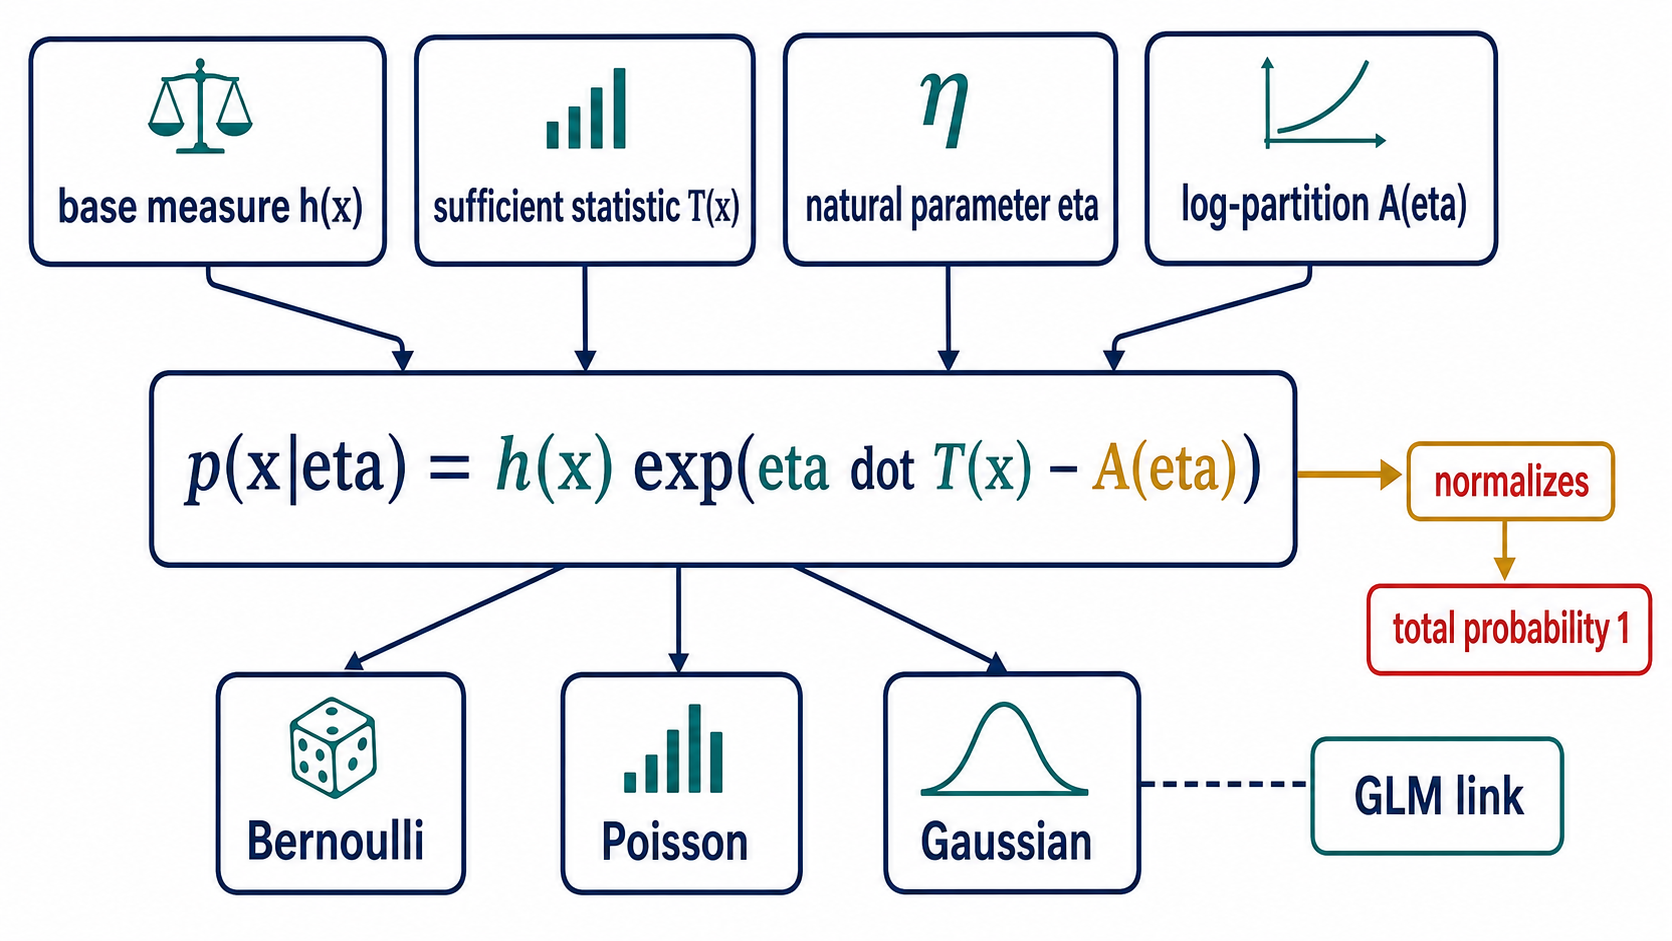
\includegraphics[width=0.98\linewidth]{imagegen-figures/ch14-exponential-family-map.png}
\caption{The exponential-family form separates the roles in a distribution. The sufficient statistic \(T(x)\) extracts data features, the natural parameter \(\eta\) weights those features, the base measure \(h(x)\) handles support-specific factors, and the log-partition function \(A(\eta)\) normalizes the result so total probability is \(1\).}
\label{fig:ch14-exponential-family-map}
\end{figure}

\paragraph{Formal setup.}
For a discrete sample space, an exponential family has PMF
\[
\boxed{
p(x\mid\eta)=h(x)\exp\!\left(\eta^\top T(x)-A(\eta)\right),
}
\]
where
\[
A(\eta)=\log\sum_x h(x)\exp\!\left(\eta^\top T(x)\right).
\]
For a continuous sample space, the sum is replaced by an integral:
\[
A(\eta)=\log\int h(x)\exp\!\left(\eta^\top T(x)\right)\,dx.
\]
The parameter values for which this quantity is finite form the natural parameter space.

For independent observations \(x_1,\ldots,x_n\), the likelihood becomes
\[
\prod_{i=1}^n p(x_i\mid\eta)
=
\left(\prod_{i=1}^n h(x_i)\right)
\exp\!\left(\eta^\top\sum_{i=1}^n T(x_i)-nA(\eta)\right).
\]
Thus the data enter the parameter-dependent part only through
\[
\sum_{i=1}^n T(x_i).
\]
This is the sufficient statistic for \(\eta\) in the independent-sample model.

\paragraph{Core intuition.}
Figure~\ref{fig:ch14-exponential-family-map} shows why the form is useful. The sufficient statistic extracts the part of the observation that matters for the parameter. The natural parameter controls how much that statistic is rewarded. The log-partition function \(A(\eta)\) is the price paid for normalization. If \(\eta\) puts more weight on large \(T(x)\), then \(A(\eta)\) must increase to keep the total probability equal to \(1\).

This form turns learning into moment matching. The model predicts an average sufficient statistic, and maximum likelihood tries to match that model average to the empirical average. This is why exponential families appear in generalized linear models: a linear predictor can produce a natural parameter, while the response distribution supplies the likelihood.

Common misconceptions: first, the natural parameter \(\eta\) may not be the familiar parameter. For Bernoulli, \(\eta\) is log-odds, not probability. For Poisson, \(\eta=\log\lambda\), not \(\lambda\). Second, \(A(\eta)\) is not an optional constant; it is essential because it depends on the parameter. Third, the clean identities below assume a regular family with support that does not change with \(\eta\). Some useful models need extra care when support depends on the parameter.

This section unifies Sections 14.1--14.3 and prepares GLMs, maximum likelihood, Bayesian conjugacy, maximum entropy, Fisher information, and information geometry.

\paragraph{Main theorem: log-partition derivatives give moments.}
Assume a regular exponential family
\[
p(x\mid\eta)=h(x)\exp\!\left(\eta^\top T(x)-A(\eta)\right)
\]
with support independent of \(\eta\). Then
\[
\boxed{\nabla A(\eta)=E_\eta[T(X)]}
\]
and
\[
\boxed{\nabla^2 A(\eta)=\operatorname{Cov}_\eta(T(X)).}
\]

\emph{Proof sketch.}
The normalization condition, written with integral notation for the continuous case and with the corresponding sum for the discrete case, is
\[
1=\int h(x)\exp\!\left(\eta^\top T(x)-A(\eta)\right)\,dx.
\]
Equivalently,
\[
e^{A(\eta)}
=
\int h(x)\exp\!\left(\eta^\top T(x)\right)\,dx.
\]
Differentiate both sides with respect to \(\eta_j\):
\[
e^{A(\eta)}\frac{\partial A}{\partial\eta_j}
=
\int T_j(x)h(x)\exp\!\left(\eta^\top T(x)\right)\,dx.
\]
Divide by \(e^{A(\eta)}\):
\[
\frac{\partial A}{\partial\eta_j}
=
\int T_j(x)h(x)\exp\!\left(\eta^\top T(x)-A(\eta)\right)\,dx
=E_\eta[T_j(X)].
\]
Stacking the components gives \(\nabla A(\eta)=E_\eta[T(X)]\). Differentiating once more gives the covariance of the sufficient statistic. In one dimension, this says
\[
A''(\eta)=\operatorname{Var}_\eta(T(X)).
\]
The mechanism is normalization: \(A(\eta)\) is exactly the function whose derivatives track how the normalized distribution's moments change.

For independent data \(x_1,\ldots,x_n\), the log-likelihood is
\[
\ell(\eta)
=
\sum_{i=1}^n \log h(x_i)
+\eta^\top\sum_{i=1}^n T(x_i)
-nA(\eta).
\]
Its gradient is
\[
\nabla\ell(\eta)
=
\sum_{i=1}^n T(x_i)-n\nabla A(\eta)
=
n\left(\overline T-E_\eta[T(X)]\right).
\]
At an interior maximum-likelihood estimate, the empirical average sufficient statistic \(\overline T\) matches the model expectation.

\paragraph{Worked examples.}
\emph{Bernoulli example.} For \(X\in\{0,1\}\),
\[
P(X=x)=\exp(\eta x-A(\eta)),
\qquad
A(\eta)=\log(1+e^\eta).
\]
The usual probability parameter is
\[
p=P(X=1)=\frac{e^\eta}{1+e^\eta}.
\]
Thus \(\eta=\log(p/(1-p))\) is the log-odds. The sufficient statistic is \(T(x)=x\). For \(n\) observations, \(\sum_i x_i\) is the number of successes.

\emph{Poisson example.} For \(X\in\{0,1,2,\ldots\}\),
\[
P(X=x)=e^{-\lambda}\frac{\lambda^x}{x!}
=\frac{1}{x!}\exp(x\log\lambda-\lambda).
\]
So
\[
h(x)=\frac{1}{x!},\qquad T(x)=x,\qquad \eta=\log\lambda,\qquad A(\eta)=e^\eta.
\]
Since \(A'(\eta)=e^\eta=\lambda\), the expected sufficient statistic is \(E[X]=\lambda\).

\emph{Gaussian with known variance.} If \(\sigma^2\) is known and \(\mu\) is unknown,
\[
p(x\mid\mu)
=\frac{1}{\sqrt{2\pi\sigma^2}}
\exp\!\left[-\frac{(x-\mu)^2}{2\sigma^2}\right].
\]
Rearrange:
\[
p(x\mid\eta)
=
\underbrace{\frac{1}{\sqrt{2\pi\sigma^2}}\exp\!\left(-\frac{x^2}{2\sigma^2}\right)}_{h(x)}
\exp\!\left(\eta x-\frac{\sigma^2\eta^2}{2}\right),
\qquad
\eta=\frac{\mu}{\sigma^2}.
\]
Thus \(T(x)=x\) and \(A(\eta)=\sigma^2\eta^2/2\). The identity \(A'(\eta)=\sigma^2\eta=\mu\) recovers the mean.

\emph{Poisson GLM example.} In a spike-count GLM, observation \(y_i\) is a spike count in time bin \(i\), and stimulus features are \(s_i\). The model sets
\[
\eta_i=w^\top s_i+b,\qquad
\lambda_i=e^{\eta_i},
\]
and
\[
\log p(y_i\mid s_i,w,b)
=y_i\eta_i-e^{\eta_i}-\log(y_i!).
\]
The sufficient statistic is the count \(y_i\), the natural parameter is the linear predictor \(\eta_i\), and the log-partition \(e^{\eta_i}\) enforces normalization.

\paragraph{ML/DL/neuroscience connections.}
Exponential families provide the likelihood layer for many models. Logistic regression uses a Bernoulli exponential family with natural parameter equal to a linear score. Multiclass classification uses a categorical exponential family with softmax normalization. Poisson regression and spike-count GLMs use a Poisson exponential family with log rate \(\eta=w^\top s+b\). Gaussian regression uses a Gaussian family for continuous residuals. Variational inference often chooses exponential-family approximate posteriors because expectations and gradients can be written in terms of sufficient statistics and log-partition derivatives. Information geometry later treats \(\eta\) and \(E[T(X)]\) as coordinate systems on a statistical manifold.

\paragraph{Exercises.}
\begin{enumerate}[label=\textbf{14.4.\arabic*.}, leftmargin=*]
\item \textbf{Mechanical.} For a Bernoulli distribution with \(p=0.8\), compute the natural parameter \(\eta=\log(p/(1-p))\).
\item \textbf{Proof or derivation.} For the Poisson exponential-family form, verify that \(A(\eta)=e^\eta\) normalizes the PMF by showing \(\sum_{x=0}^\infty \frac{1}{x!}\exp(\eta x-e^\eta)=1\).
\item \textbf{Numerical/computational.} In a Poisson GLM, let \(\eta=1.2\). Compute the predicted rate \(\lambda=e^\eta\) approximately, and write the log-likelihood contribution for observing \(y=3\).
\item \textbf{Interpretation.} For independent Bernoulli data, why is the number of successes sufficient for estimating \(p\)? What information about the sequence order is irrelevant under the model?
\item \textbf{Debug the misconception.} A student says, "The exponential family is just the exponential distribution." Use Bernoulli or Poisson to explain why this is false.
\end{enumerate}

\paragraph{Closing bridge.}
Chapter 14 organized common distributions by support, story, parameters, and sufficient statistics. The next chapter turns these distributions into prediction machinery. Expectations average functions under a distribution, conditioning updates distributions when information arrives, and Bayes' theorem reweights hypotheses by their likelihoods. Later chapters will use the same distributions as likelihoods for inference, as approximations in high dimensions, and as geometric objects whose distinguishability can be measured.

\clearpage
